\section{EXCELLENCE}
\label{sec:excellence}

\subsection{Quality and credibility of the research/innovation action}
\label{sec:quality}

\subsubsection{Introduction}
\label{sec:introduction}

In Europe, prostate cancer is reported to be the most frequently diagnosed cancer among men and thus one of the leading causes of death of cancer~\footcite{Ferlay2013}. 
Currently, addressing this issue is a major public debate, where the implementation of appropriate screening methods and subsequent treatments is key.
In this regard, the \ac{erspc} is conducted to investigate the potential benefits of a population-based screening~\footcite{Schroder2015}. 
The screening consists of a \ac{psa} test and depending of the \ac{psa} level measured, an additional ``blind'' biopsy is carried out. 
Despite that mortality significantly has been decreasing, the employed screening strategy suffers of a high rate of over-diagnosis and over-treatment~\footcite{Delpierre2013}, and misses the more aggressive cancers in the \ac{cg}.
%, due to the fact that prostate cancers grow either slowly or fast.
%The slow-growing tumours account for up to~85~\% of all cancers and stay confined to the prostate gland, while the fast-growing tumours rapidly develop and metastasise to other organs, significantly affecting the morbidity and mortality rate.
%Furthermore, prostate cancer is more likely to develop in specific regions of the prostate: around~70-80~\% of prostate cancers originate in the \ac{pz}, whereas~10-20~\% in the \ac{cg}, but are more aggressive and more likely to invade other organs. 
\textbf{Thus, additionally to cancer detection, the screening methods need to estimate the cancer aggressiveness to allow clinicians to act accordingly.}

In addition, the investigators of the \ac{erspc} have concluded that the use of \emph{``multi-parametric \ac{mri} and the development of new markers are the hope for the future''}.
That is why, \ac{cad} systems, revolved around mono- and currently multi-parametric \ac{mri} are developed by the medical imaging community, and have given rise to the field of \textbf{radiomics} consisting in automatically extracting large a number of quantitative features~\footcite{lambin2012radiomics}.
Recently, Lema\^itre~\emph{et al.} extensively reviewed the developed \ac{cad} systems for prostate cancer detection~\footcite{Lemaitre2015}.
The developed \ac{cad} systems are designed under the same architecture composed of: (i) pre-processing, (ii) registration-segmentation, (iii) feature detection, (iv) feature extraction/selection, and (v) feature classification.
% as depicted in Fig.\,\ref{fig:wkfcad}. 
The available \ac{mri} modalities during prostate exam are \ac{t2w}-\ac{mri}, \ac{dw}-\ac{mri}, \ac{dce}-\ac{mri}, and \ac{mrsi}. 
Additionally, \ac{adc} map is based on the computation of a coefficient derived from multiple \ac{dw}-\ac{mri} acquisition.
\textbf{Currently, no \ac{cad} system has been developed using all the available imaging modalities and taking into account the radiomics signature but they discarded their potential for discriminating power to diagnose prostate cancer.}
The closest attempts have used three of these modalities (i.e., \ac{t2w}-\ac{mri}, \ac{dw}-\ac{mri}, \ac{dce}-\ac{mri}) and have discarded \ac{mrsi}~\footcite{Litjens2014}\textsuperscript{,}\footcite{Viswanath2011}.
This latter, however, has been shown to be extremely helpful to grade cancer aggressiveness particularly in the \ac{cg}~\footcite{Vos2015}, which is the most challenging zone in terms of cancer detection.
\textbf{Furthermore, the current research mainly focus on the delineation of prostate cancers rather than on the cancer aggressiveness assessment.}

% \begin{figure*}[h]
  \centering

  % Define block styles used later

  \tikzstyle{module}=[draw, draw=blue!80, text width=10em, 
  text centered, minimum height=5em, minimum width = 15em, drop shadow, rounded corners,
  fill=blue!30]
  
  \tikzstyle{vecArrow} = [thick, decoration={markings,mark=at position
    1 with {\arrow[semithick]{open triangle 60}}},
  double distance=1.4pt, shorten >= 5.5pt,
  preaction = {decorate},
  postaction = {draw,line width=1.4pt, white,shorten >= 4.5pt}]

  % Define distances for bordering
  \def\blockdist{1.5}
  \def\edgedist{2.5}

  \begin{tikzpicture}[node distance=3cm,thick,scale=0.4, every node/.style={scale=0.4},path image/.style={
      path picture={
        \node at (path picture bounding box.center) {
          \includegraphics[width=1cm]{#1}
        };}}]
    \tikzstyle{conefill} = [path image=,fill opacity=0.8]
    \node[module=above:pre] (pre) at (4.5,-2.6) {\Large Pre-processing};
    \node[module,below of=pre] (seg) {\Large Segmentation};
    \node[module,below of=seg] (reg) {\Large Registration};

    \path[->,dashed] (seg.west) edge [bend right=70] node {} (reg.west);
    \path[->,dashed] (reg.east) edge [bend right=70] node {} (seg.east);

    \draw[->] (pre)--(seg);
    \draw[->] (seg)--(reg);

    \begin{pgfonlayer}{background}
      \path (pre.west |- pre.north)+(-0.9,1.0+\blockdist) node (a) {};
      \path (reg.east |- reg.south)+(+0.9,-0.5) node (b) {};
      
      \path[fill=blue!10,rounded corners, draw=blue!20, dashed] (a) rectangle (b);
    \end{pgfonlayer}
    
    \path (pre.north) +(0,+\blockdist) node (bgreg) {\Large Image regularization};

    \begin{scope}[node distance=10cm]
      \node[module] (det) [below right=0cm and 3cm of pre] {\Large Features detection};
    \end{scope}
    \begin{scope}[node distance=3.5cm]
      \node[module,above of=det] (roi) {\Large ROIs\\detection/selection};
    \end{scope}
    \node[module,below of=det] (sel) {\Large Features\\selection/extraction};
    \node[module,below of=sel] (cla) {\Large Features\\classification/fusion};

    \draw[->] (roi)--(det);
    \draw[->] (det)--(sel);
    \draw[->] (sel)--(cla);

    \begin{pgfonlayer}{background}
      \path (roi.west |- roi.north)+(-0.25,0.8) node (c) {};
      \path (roi.east |- roi.south)+(+0.25,-0.25) node (d) {};
      
      \path[fill=blue!20,rounded corners, draw=blue!25, dashed] (c) rectangle (d);
    \end{pgfonlayer}

    \path (roi.west |- roi.north) +(.6,0.4) node (bgfea) {\Large \textbf{CADe}};

    \begin{pgfonlayer}{background}
      \path (det.west |- det.north)+(-0.25,0.8) node (c) {};
      \path (cla.east |- cla.south)+(+0.25,-0.25) node (d) {};
      
      \path[fill=blue!20,rounded corners, draw=blue!25, dashed] (c) rectangle (d);
    \end{pgfonlayer}

    \path (roi.west |- det.north) +(.6,0.4) node (bgfea) {\Large \textbf{CADx}};     

    % Define the place where the arrow should start anf finish
    \path (seg.east |- seg.north)+(+0.9,0) node (e) {};
    \path (sel.west |- seg.north)+(-0.8,0) node (f) {};

    \draw[double distance =3pt,preaction={-triangle 90,thin,draw,shorten >=-1mm}] (e) -- (f) node[midway,above] {\Large Regularized data};

    \begin{scope}[yshift=34,xshift=-86]
      \transparent{0.6}\draw[path image=content/proposal/figures/tikzimage/t2.eps] (0,0) rectangle (1.0,1.0);
    \end{scope}

    \begin{scope}[yshift=31,xshift=-83]
      \transparent{0.6}\draw[path image=content/proposal/figures/tikzimage/t2.eps] (0,0) rectangle (1.0,1.0);
    \end{scope}

    \begin{scope}[yshift=28,xshift=-80]
      \transparent{0.8}\draw[path image=content/proposal/figures/tikzimage/t2.eps] (0,0) rectangle (1.0,1.0);
      \path (0,0)+(-1.5,0.3) node {\Large T$_2$-W MRI};
    \end{scope}

    \begin{scope}[yshift=-33,xshift=-86]
      \transparent{0.6}\draw[path image=content/proposal/figures/tikzimage/t2.eps] (0,0) rectangle (1.0,1.0);
    \end{scope}

    \begin{scope}[yshift=-36,xshift=-83]
      \transparent{0.6}\draw[path image=content/proposal/figures/tikzimage/t2.eps] (0,0) rectangle (1.0,1.0);
    \end{scope}

    \begin{scope}[yshift=-39,xshift=-80]
      \transparent{0.8}\draw[path image=content/proposal/figures/tikzimage/t2.eps] (0,0) rectangle (1.0,1.0);
      \path (0,0)+(-1.2,0.3) node {\Large T$_2$ map};
    \end{scope}

    \begin{scope}[yshift=-100,xshift=-86]
      \transparent{0.6}\draw[path image=content/proposal/figures/tikzimage/dce.eps] (0,0) rectangle (1.0,1.0);
    \end{scope}

    \begin{scope}[yshift=-103,xshift=-83]
      \transparent{0.6}\draw[path image=content/proposal/figures/tikzimage/dce.eps] (0,0) rectangle (1.0,1.0);
    \end{scope}

    \begin{scope}[yshift=-106,xshift=-80]
      \transparent{0.8}\draw[path image=content/proposal/figures/tikzimage/dce.eps] (0,0) rectangle (1.0,1.0);
      \path (0,0)+(-1.5,0.3) node {\Large DCE MRI};
    \end{scope}

    \begin{scope}[yshift=-167,xshift=-86]
      \transparent{0.6}\draw[path image=content/proposal/figures/tikzimage/dwi1.eps] (0,0) rectangle (1.0,1.0);
    \end{scope}

    \begin{scope}[yshift=-170,xshift=-83]
      \transparent{0.6}\draw[path image=content/proposal/figures/tikzimage/dwi1.eps] (0,0) rectangle (1.0,1.0);
    \end{scope}

    \begin{scope}[yshift=-173,xshift=-80]
      \transparent{0.8}\draw[path image=content/proposal/figures/tikzimage/dwi1.eps] (0,0) rectangle (1.0,1.0);
      \path (0,0)+(-1.5,0.3) node {\Large DW MRI};
    \end{scope}

    \begin{scope}[yshift=-234,xshift=-86]
      \transparent{0.6}\draw[path image=content/proposal/figures/tikzimage/adc.eps] (0,0) rectangle (1.0,1.0);
    \end{scope}

    \begin{scope}[yshift=-237,xshift=-83]
      \transparent{0.6}\draw[path image=content/proposal/figures/tikzimage/adc.eps] (0,0) rectangle (1.0,1.0);
    \end{scope}

    \begin{scope}[yshift=-240,xshift=-80]
      \transparent{0.8}\draw[path image=content/proposal/figures/tikzimage/adc.eps] (0,0) rectangle (1.0,1.0);
      \path (0,0)+(-1.5,0.3) node {\Large ADC};
    \end{scope}

    \begin{scope}[yshift=-301,xshift=-86]
      \transparent{0.6}\draw[path image=content/proposal/figures/tikzimage/mrsi.eps] (0,0) rectangle (1.0,1.0);
    \end{scope}

    \begin{scope}[yshift=-304,xshift=-83]
      \transparent{0.6}\draw[path image=content/proposal/figures/tikzimage/mrsi.eps] (0,0) rectangle (1.0,1.0);
    \end{scope}

    \begin{scope}[yshift=-307,xshift=-80]
      \transparent{0.8}\draw[path image=content/proposal/figures/tikzimage/mrsi.eps] (0,0) rectangle (1.0,1.0);
      \path (0,0)+(-1,0.3) node {\Large MRSI};
    \end{scope}

    \path (pre.west |- roi.north)+(-3.5,1.0+\blockdist) node (g) {};
    \path (reg.west |- cla.south)+(-3.5,-0.5) node (h) {};

    \draw[decorate,decoration={brace,raise=6pt,amplitude=10pt}, thick]
    (g)--(h) ;
    
    \path (seg.west |- seg.north)+(-2.5,0) node (i) {};
    \path (seg.west |- seg.north)+(-0.9,0) node (j) {};
    
    \draw[double distance =3pt,preaction={-triangle 90,thin,draw,shorten >=-1mm}] (i) -- (j);   

    \path (sel.east |- seg.north)+(2,0) node (k) {};
    \path (sel.east |- seg.north)+(0.5,0) node (l) {};
    
  \end{tikzpicture}
  \caption{Common \ac{cad} framework based on \ac{mri} images used to detect prostate cancer.}
  \label{fig:wkfcad}
\end{figure*}

% \begin{figure*}
%   \centering
%   \hspace*{\fill}
%   \subfigure[\ac{t2w}-\ac{mri} slice of an healthy prostate acquire with a 1.5 Tesla \ac{mri}. The blue contour represents the \ac{cg} while the \ac{pz} corresponds to the green contour.]{\label{subfig:t2whealthy}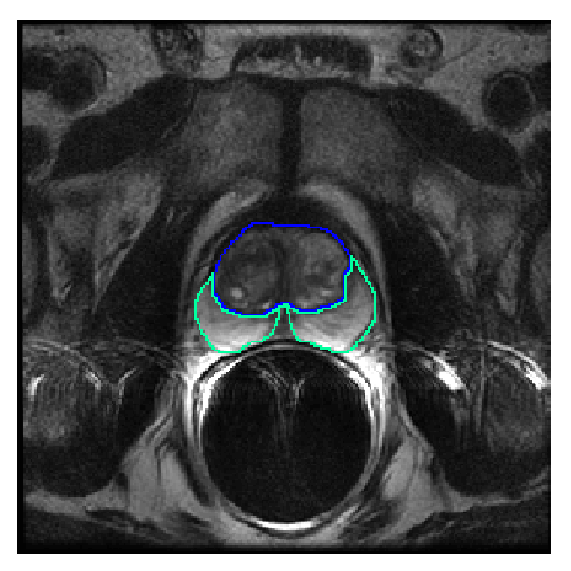
\includegraphics[width=0.3\linewidth]{12_figures/figures/t2w/t2w_healthy.eps}} \hfill
%   \subfigure[\ac{t2w}-\ac{mri} slice of a prostate with a \ac{cap} highlighted in the \ac{pz} using a 3.0 Tesla \ac{mri} scanner.]{\label{subfig:t2wcancerpz}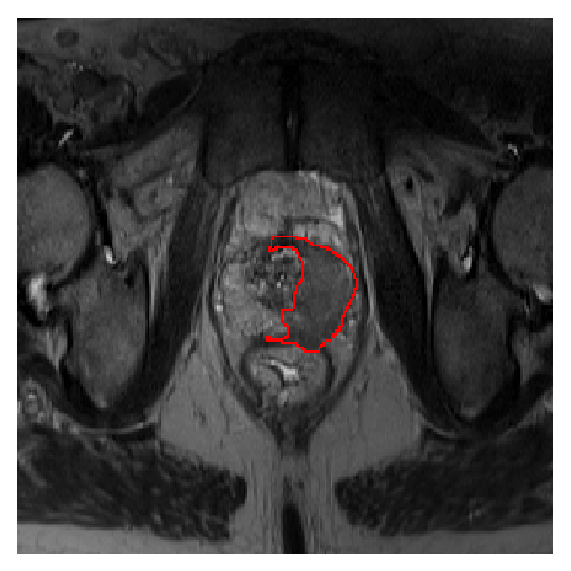
\includegraphics[width=0.3\linewidth]{12_figures/figures/t2w/t2w_cancer_pz.eps}} \hfill
%   \subfigure[\ac{t2w}-\ac{mri} slice of a prostate with a \ac{cap} highlighted in the \ac{cg} using a 3.0 Tesla \ac{mri} scanner.]{\label{subfig:t2wcancercg}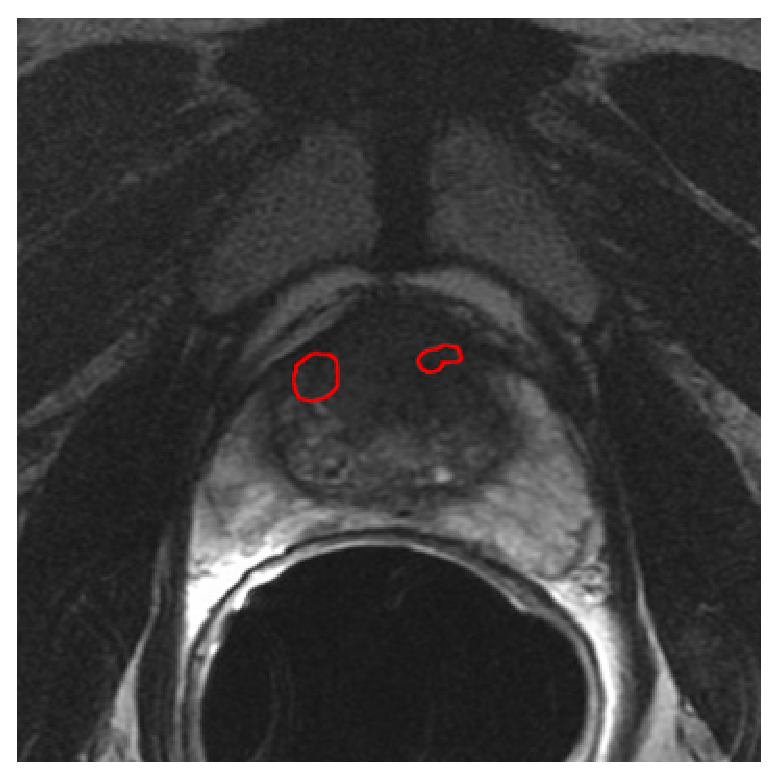
\includegraphics[width=0.3\linewidth]{12_figures/figures/t2w/t2w_cancer_cg.eps}}
%   \hspace*{\fill}
%   \caption{Rendering of \ac{t2w}-\ac{mri} prostate image with both 1.5 and 3.0 Tesla \ac{mri} scanner.}
%   \label{fig:t2w}
% \end{figure*}

% \begin{figure*}
%   \centering
%   \hspace*{\fill}
%   \subfigure[]{\label{subfig:t1w}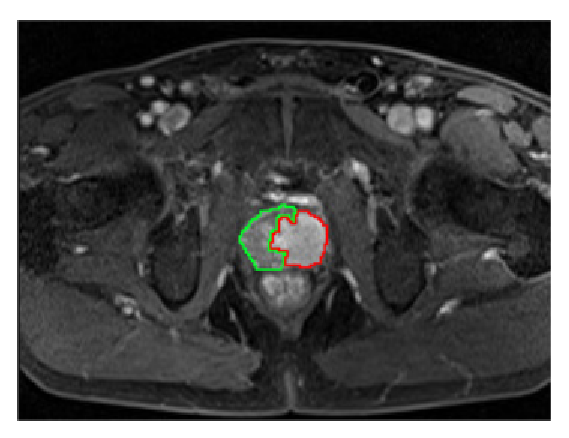
\includegraphics[width=0.35\linewidth]{12_figures/figures/dce/slice.eps}} \hfill
%   \subfigure[]{\label{subfig:dce}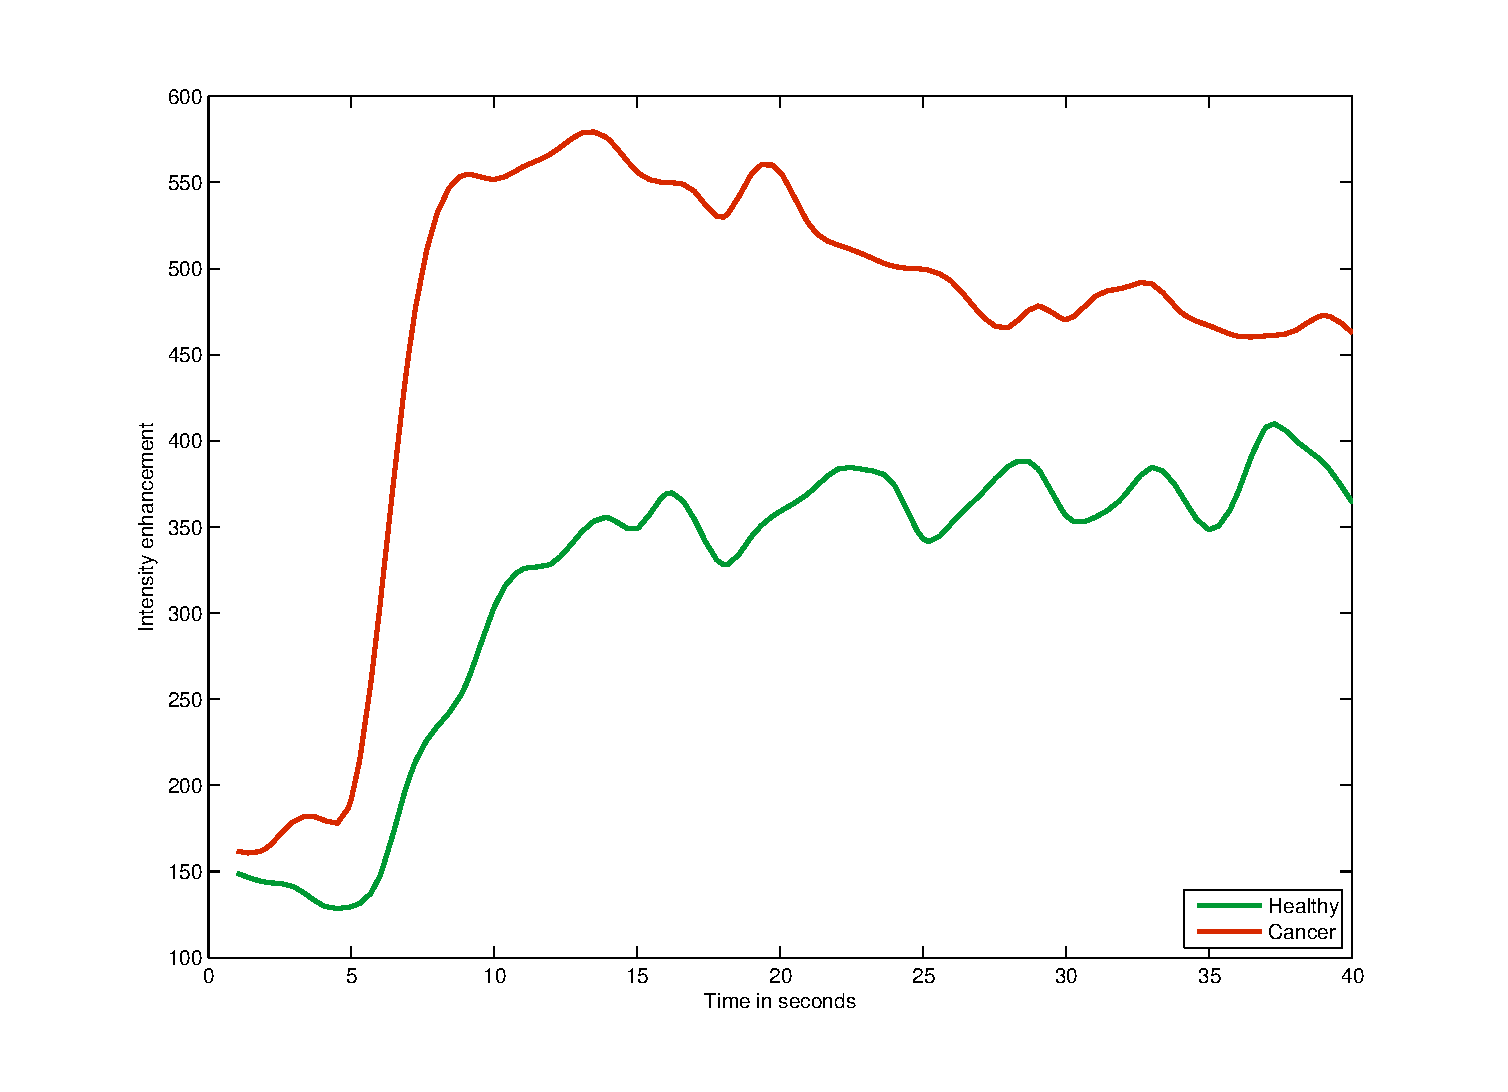
\includegraphics[width=0.35\linewidth]{12_figures/figures/dce/dce_cancer_healthy.eps}}
%   \hspace*{\fill}
%   \caption{Illustration of: \subref{subfig:t1w} \ac{t1w}-\ac{mri} image and \subref{subfig:dce} typical enhancement signals observed in \ac{dce}-\ac{mri} analysis collected with a 3.0 Tesla \ac{mri} scanner. The red curve is typical from \ac{cap} while the green curve is characteristic of healthy tissue.}
%   \label{fig:dceana}
% \end{figure*}

% \begin{figure}
%   \centering
%   \hspace*{\fill}
%   \subfigure[]{\label{subfig:dwi}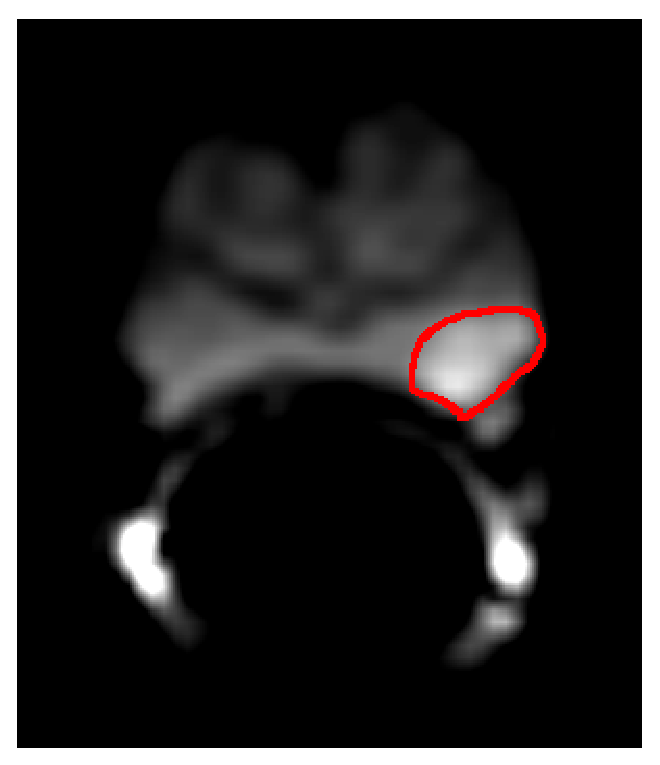
\includegraphics[height=0.15\textheight]{12_figures/figures/dwi/dwi_cancer.eps}} \hfill
%   \subfigure[]{\label{subfig:adc}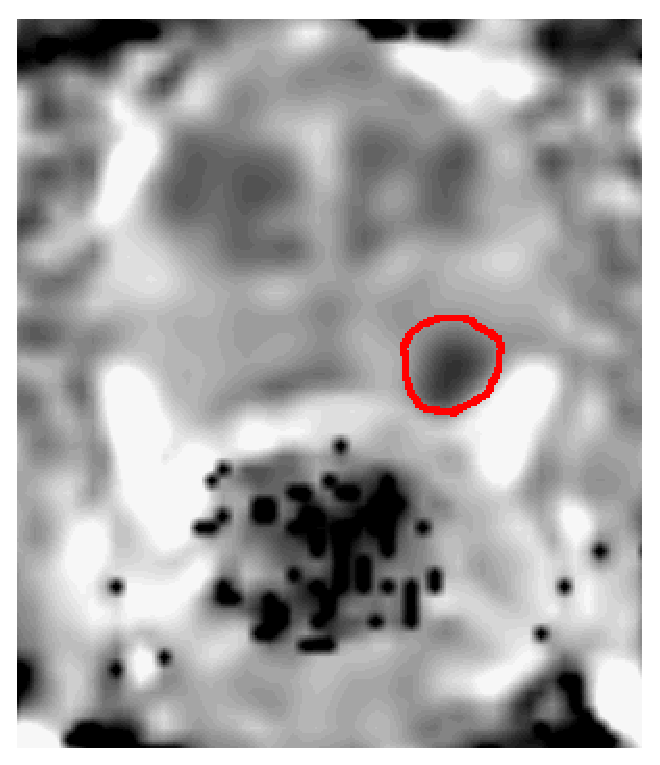
\includegraphics[height=0.15\textheight]{12_figures/figures/dwi/adc_cancer.eps}}
%   \hspace*{\fill}
%   \caption{Illustration of: \subref{subfig:dwi} \ac{dw}-\ac{mri} and \subref{subfig:adc} \ac{adc} map. The signal intensity corresponding to cancer are inversely correlated on these two types of imaging techniques. The cancer is highlighted in red.}
%   \label{fig:dwi}
% \end{figure}

% \begin{figure*}
%   \centering
%   \hspace*{\fill}
%   \subfigure[]{\label{subfig:mrsihea}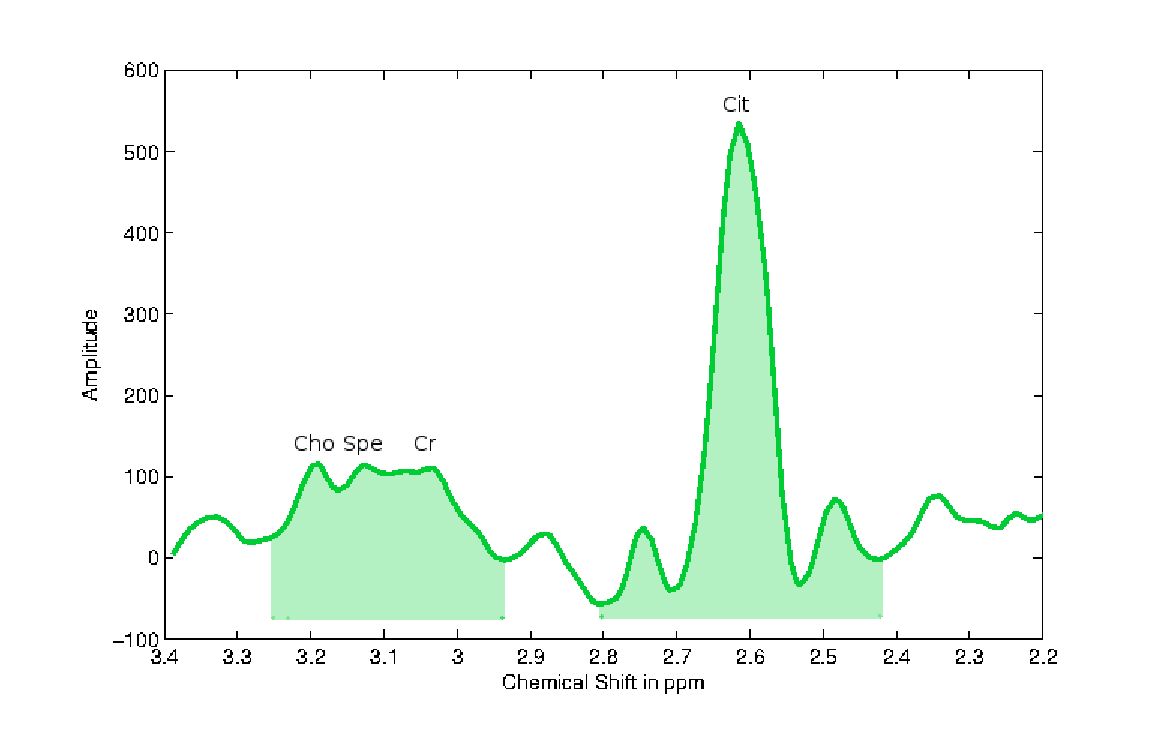
\includegraphics[width=0.45\linewidth]{12_figures/figures/mrsi/mrsi_healthy.eps}} \hfill
%   \subfigure[]{\label{subfig:mrsican}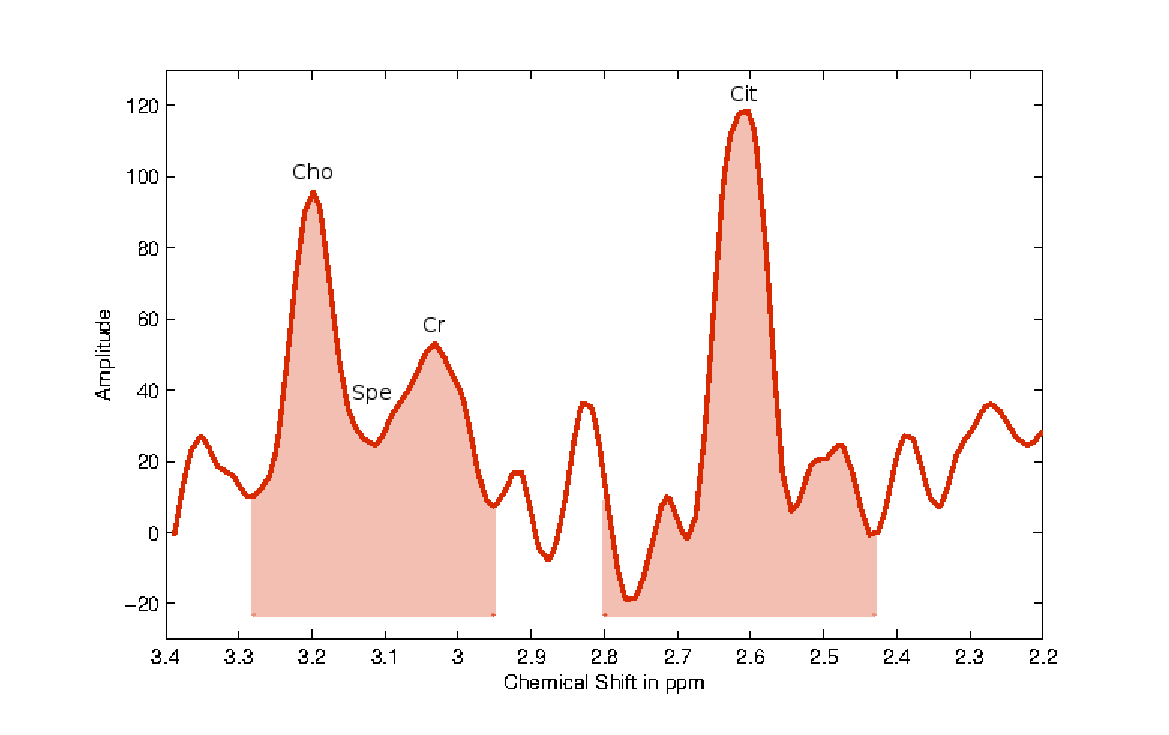
\includegraphics[width=0.45\linewidth]{12_figures/figures/mrsi/mrsi_cancer.eps}}
%   \hspace*{\fill}
%   \caption{Illustration of an \ac{mrsi} spectrum both \subref{subfig:mrsihea} healthy and \subref{subfig:mrsican} cancerous voxel with a 3.0 Tesla \ac{mri}. The highlighted areas corresponds to the related concentration of the metabolites which is computed by integrating the area under each peak. Acronyms: Choline (Cho), Spermine (Spe), Creatine (Cr) and Citrate (Cit).}
%   \label{fig:mrsi}
% \end{figure*}

%%% Local Variables: 
%%% mode: latex
%%% TeX-master: "../../../main"
%%% End: 


Therefore, the aim of this project is to design a \ac{cad} system able to both detect and assess prostate cancers using all currently available multi-parametric \ac{mri} modalities and the radiomics paradigm, by analyzing different automated and traditional imaging features.
%To achieve this goal, we will revisit the different stages of the \ac{cad} framework.
%First, we will insure to work with the most consistent data, enhancing them using different types of pre-processing.
%Subsequently, we will segment the prostate zones using multi-parametric \ac{mri} images 

% {\color{red} drastically improve here
% The architecture of our \ac{cad} system will imply the following investigations: 
% \begin{enumerate}
% \item Pre-processing to enhance the quality of \ac{mri} images (bias field correction, denoising, and normalisation),
% \item Segmentation of prostate zones using multi-parametric \ac{mri} and deep-learning,
% \item Registration of multi-parametric \ac{mri} using spline-based non-linear differmorphism,
% \item Detection and assessment of prostate cancers using using multi-parametric \ac{mri} and deep-learning,
% \item Identification of markers by inspection of the neural-network and transfer to classical machine learning approach.
% \item Grading using standard PI-RADS
% \end{enumerate}
% }
%These methodologies will be extensively presented and argued in Sect.\,\ref{sec:methodologies}.

\subsubsection{Research methodologies}
\label{sec:methodologies}

\paragraph{Data acquisition}

The unavailability of a public dataset in medical imaging is a major drawback.
Currently, no multi-parametric \ac{mri} prostate data are publicly available, implying that no fair comparisons can be drawn between the different developed \ac{cad} systems.
Recently, Lema\^itre~\emph{et al.} have launch a beta web-platform~\footnote{\texttt{http://i2cvb.github.io/}} intended for reporting the evaluation of \ac{cad} systems.
A multi-parametric \ac{mri} dataset is made available, containing 60 patients and the following modalities: \ac{t2w}-\ac{mri}, \ac{dw}-\ac{mri}, \ac{dce}-\ac{mri}, and \ac{mrsi}.
Furthermore, the data are acquired from both 1.5 T and 3.0 T \ac{mri} scanner.
Multiple ground-truths (i.e., prostate zones, cancer lesions) are compiled by experienced radiologists and additional biopsy tests.
However, the web-platform needs to be completed before being made fully available.
\textbf{Consequently, we will finalise the dataset and release it publicly through our web-platform.}

\paragraph{Pre-processing}

\Ac{mri} images are corrupted by different phenomena: (i) bias field, (ii) noise, and (iii) inter-patient variations.
In this regard, particular attention to correct each of these drawbacks will be given.

\Ac{mri} images are affected by the inhomogeneity of the \ac{mri} field called bias field, resulting in a smooth variation of the intensities across each image.
Although bias correction methods are commonly used to enhance brain \ac{mri} images~\footcite{Vovk2007}, only one \ac{cad} system for prostate has reported to use such pre-processing~\footcite{Viswanath2009}.
The same authors have empirically evaluated the state-of-the-art methods~\footcite{viswanath2011empirical} concluding that N3 algorithm~\footcite{Sled1998} yields to better classification performance than other methods.
Recently, Lin~\emph{et al.}~\footcite{Lin2011} have proposed a method combining the N3 algorithm with the Fuzzy C-Means algorithm which outperforms the original methods, in terms of breast segmentation.
\textbf{Therefore, we will compare these state-of-the-art methods, by ensuring the benefit of the method of Lin~\emph{et al.} for our specific application.}

Apart from the bias field, \Ac{mri} images are also degraded by a Rician noise. 
Similarly to bias correction, only two \ac{cad} systems have filtered the images using wavelet-based techniques~\footcite{Mallat2008}\textsuperscript{,}\footcite{Pizurica2003}, which offer a proper theoretical baseline for Rician corruption~\footcite{Nowak1999}.
Non-Local Means-based denoising techniques have extensively and successively been used for other \ac{mri} applications, but never for \ac{mri} prostate images.
\textbf{Thus, we will evaluate the Non-Local Means-based techniques~\footcite{Manjon2012} and wavelet-based technique to select the appropriate method for our application.}

%\ac{cad} systems are based on machine learning classifiers which are trained to differentiate cancerous from healthy tissue.
%The classification performance of these classifiers highly relies on the consistency of the dataset.
%Subsequently, one can emphasize the desire to reduce the inter-patient variability of the \ac{mri} dataset.
%In this regard, each patient dataset needs to be standardised/normalised to a common basis, modality by modality.
Only two methods have been used in \ac{cad} for prostate to reduce the inter-patient variability in the \ac{mri} dataset: the first method consists in normalising the images via the $z$-score, while the second technique is based on a linear normalisation by parts~\footcite{Madabhushi2006a}.
Lema\^itre~\emph{et al.} have developed a normalisation technique using the Rician properties of the \ac{mri} signal~\footcite{lemaitre2016normalization}, which outperforms the previous methods for \ac{t2w}-\ac{mri} images.
Furthermore, Lema\^itre~\emph{et al.} have developed a method to standardized \ac{dce}-\ac{mri} data, showing the benefit when detecting prostate cancer in comparison with un-normalized data and quantitative methods.
\textbf{Thus, we will extend this work to \ac{dw}-\ac{mri} modalities and on larger cohort of patient to test the reliability of these methods.}

\ac{mrsi} is a modality related to one dimensional signal, and the enhancing techniques differ from the one used in \ac{mri}.
The \ac{mrsi} spectra have to be corrected for several phenomena: phase correction, water and lipid residuals filtering, baseline correction, frequency alignment, and normalisation.
This set of enhancement techniques has already been investigated by Lema\^itre~\emph{et al.} in a study focusing solely on the \ac{mrsi} modality for prostate cancer detection~\footcite{Lemaitre2011}; \textbf{this knowledge will be the basis of \ac{mrsi} enhancement.}

\paragraph{Segmentation}

To achieve robust cancer detection, the classification has to be carried out only in the prostate area, motivating the need to perform a segmentation of the organ in the \ac{mri} images.
Furthermore, as mentioned in Sect.\,\ref{sec:introduction}, the \emph{a-priori} membership of a voxel to belong to a zone (i.e., \ac{pz} or \ac{cg}) has a high potential to increase the performance to assess the aggressiveness of prostate cancer.
Therefore, the prostate zones need to be segmented instead of solely the prostate organ.
%In this regard, the work of Litjens~\emph{et al.} have segmented the prostate zones using a probabilistic multi-atlas approach~\footcite{Litjens2014a}.
Previous segmentation methods only used \ac{t2w}-\ac{mri} modality and sometimes \ac{adc} map.
%Although atlas-based methods are robust to intensity variations, they lack accuracy in the boundary delineations~\footcite{Ghose2012}.
%The potential of machine learning methods to carry out such a task is currently underestimated, but has been shown to be suitable in combination with the other approaches (i.e., deformable models or atlas-based)~\footcite{ghose2012graph}.
\textbf{Thus, we will design a hybrid system to segment the prostate zones, based on \ac{cnn} and \ac{asm} using all multi-parametric images.}
The choice of \ac{cnn} is motivated by the recent breakthrough of deep-learning in multiple fields of computer vision.
Deep-learning, however, has still not been extensively used in the field of medical imaging.
% as attested by the organisation of the first workshop specifically dedicated to this topic at MICCAI 2015. 
%Deep-learning relies on a data-driven training stage in which large amounts of data are required, which is a serious drawback in medical imaging.
%However, this problem is addressed by transfer learning which allows deep-learning applied to medical imaging.

\paragraph{Registration}

In multi-parametric \ac{mri}, the data are collected in a sequential manner, involving a possible misalignment between the different modalities.
Mitra~\emph{et al.} developed an automatic multi-modal non-rigid registration method~\footcite{Mitra2012a}, which has been shown to outperform the state-of-the-art methods.
This method has initially been used for registration between \ac{t2w}-\ac{mri} and \ac{us} prostate images; \textbf{therefore, we will extend this method to align our multi-parametric \ac{mri} dataset.}

\paragraph{Detection and assessment}

Up to now, \ac{cad} developed systems have solely focused on the detection of prostate cancers, omitting a real assessment of the lesion aggressiveness.
The detection of cancers is commonly performed using machine learning classifiers, designing frameworks relying on two compulsory stages and an intermediate optional one: (i) features detection, (ii) features selection/extraction and (iii) features classification.
Lema\^itre~\emph{et al.} have extensively reviewed research carried out in each of this stage for the development of \ac{cad} for prostate cancer~\footcite{Lemaitre2015}.
%These stages are organised in a sequential manner and thus stages upstream part of the features classification have a tremendous importance on the classification performance.
Consequently, the use of discriminative features is certainly key and most probably the bottleneck of \ac{cad} systems, justifying the attention given by researchers to evaluate a multitude of low- and high-level visual features, inspired by computer vision or human perception.
Deep-learning has been recently shown to be one of the most successful machine learning techniques in broad types of classification tasks.
\ac{cnn} has the ability to generate automatically low- and high-level visual features in the network itself~\footcite{Zeiler2013} by only supplying the raw data as inputs.
Additionally, \ac{cnn} might be considered as a good candidate to automatically generate large number of features, which can be later analyzed.
Furthermore, \ac{cnn} can be trained using the Gleason grade obtained through biopsy in order to get an assessment of the aggressiveness of the cancer.
\textbf{Thus, we will detect and assess prostate cancers with \ac{cnn} and validate the classifier using \ac{roc} analysis.
  In addition, we will investigate the low- and high-level features to find potential new markers which can be used by clinicians or other machine learning methods as the basis for radiomics applied to prostate cancer.}

\paragraph{Evaluation using \acs*{pirads}}

The \ac{esur} together with the \ac{acr} have recently published the \ac{pirads}, which is the standard way to assess and report prostate lesions using multi-parametric \ac{mri}.
This standard allows to assign a score depending on multiple criteria such as signal intensity, texture, size of lesion, modality, prostate zones, etc.
None of the current \ac{cad} systems offer a \ac{pirads} score when detecting potential lesions in multi-parametric \ac{mri}.
\textbf{Thus, we will report the output of our classification framework in terms of \ac{pirads} score, applying the provided criterion.}

\subsubsection{Originality and innovative aspects of the research programs}

In response to the urgent needs that the medical community is facing, the principal investigators seek to address the grand challenge in the \textbf{early detection and accurate assessment} of prostate cancer by (i) developing an advanced \ac{cad} system based on novel image analysis and data mining techniques and \textbf{\ac{pirads}} scores, and (ii) evaluating and validating it in the clinical practise. 
Mining imaging features in a non-invasive and cost-effective way is known as \textbf{radiomics}.
The central premise this study is that these imaging features quantify phenotypic characteristics of the entire tumour and reflect the underlying gene and protein expression patterns.
\textbf{Correct decoding of the radiomics signature of prostate cancer in multi-parametric \ac{mri} may allow differentiation between lethal and non lethal prostate cancers in a non invasive manner at the time of detection.}
This project will revolutionize prostate cancer screening by increasing its efficacy and decreasing negative side effects.
PREDICATE will serve as a blueprint for screening and diagnosis of other cancers.

\subsection{Quality and appropriateness of the training and of the two way transfer of knowledge between the researcher and the host}
\label{sec:transfer}

The main objective of the present project is to establish a mutually beneficial partnership between the host institute, the \ac{fsu}, the fellow and the beneficiary, the \ac{udg}, with the goal to develop the first multi-parametric \ac{cad} system for prostate cancer detection and diagnosis.
The proposed research will allow the fellow to continue gaining experience in his former research line, the design of multi-parametric \ac{cad} systems portable to many other cancers such as breast and brain.
The fellow will gain expertise in developing intelligent \ac{cad} systems, novel pre-processing techniques to be applied to prostate images and integrated in the \ac{cad} system, and in cancer research in general.

At the start of his training in \ac{fsu}, G. Lema\^itre will be required to attend an \textbf{orientation session hosted by the \ac{opa}}, which will provide information on postdoctoral policies, campus resources (e.g., libraries, computing facilities, grants office), and coursework, teaching, and funding opportunities.
\ac{fsu} currently offers a \textbf{postdoctoral seminar series} at which postdocs can present and receive feedback on their research, as well as courses in pedagogy, grants management, organizational behavior, and the structure of colleges and universities.
\ac{fsu} also has several certificate programs aimed at providing additional training to postdocs.
For example, the \textbf{Postdoctoral Certificate Program in Research} offers coursework in research ethics, mentoring, and becoming an independent investigator, as well as traditional journal club and research training experiences.
\ac{fsu} has an \textbf{biannual Industry Day} where medical companies present their research and PhD students and postdocs as well and new research lines can be exchanged and established.
The host's department has two visiting professors in radiology, Prof. K. Pinker-Domenig and M. Lobbes, specialized in prostate research who have strong connections to \textbf{General Electric, Philips, and Siemens}, which will help the fellow in the development of adequate \ac{cad} solution for clinicians.
The close proximity of the \textbf{Lee-Moffitt-Cancer Center}, the biggest in the Southeast of US, and the strong ties to \textbf{MD Anderson} ensure an additional link to the cutting edge clinical research in prostate cancer.
\ac{opa} also regularly hosts career development seminars, to which the fellow will participate, on topics such as grant writing, lab management, research ethics, networking and interviewing, and teaching, and it has staff experienced at providing career advising suited to biomedical science researchers.

At both \ac{fsu} and \ac{udg}, G. Lemai\^itre will participate actively in weekly group meetings discussing current literature, grant applications, manuscripts, and programming/algorithmic problems.
Additionally, G. Lema\^itre will mentor PhD students together with Prof. A. Meyer-Baese and Dr. R. Mart\'i.
Furthermore, they will transfer to the fellow additional skills which they gain during their research years such as: algorithm implementation; mathematical modelling; ability to attract funding; expertise as editor of books and journal special issues; and student tutoring, curriculum development, and doctoral committee chair.
Prof. A. Meyer-Baese will also share her expertise in clinical domain: patient management; understanding cutting-edge medical methods and techniques; collaborating with physicians; radiological sources and MR images management; database management, storage and processing.

In the outgoing phase, it should be emphasize that the young and active research group computer vision and robotic (ViCOROB), to which the host institution in Europe belongs, will definitely benefit from this project in the incoming phase, capitalising on the works carried out for the last decade in the area of prostate cancer. The fellow will play an indispensable role in the group by: training new researchers, superivising PhD candidates and MSc students, attracting for funding, applying for new grants/projects,  establishing collaborations with other groups, contacting industry related agents, strengthen hospitals and health services relations, participating in seminars, publishing papers, and attending to conferences.

Finally, G. Lema\^itre is the perfect candidate for the propose challenge related to the transfer of knowledge between two international institutions as \ac{udg} and \ac{fsu}: although G. lema\^itre is a junior scientist, he successfully tackled the challenge of working interdisciplinary with two research groups located in two different countries during his joint PhD at \ac{udg} and \ac{ub}, to which he successfully met as his research records show.
Furthermore, he already proved is competence to perform delocalized research has shown by his enrolment in the open-source software community, by collaborating with researchers from different institutions\footnote{\texttt{https://github.com/scikit-learn-contrib/imbalanced-learn}}.
Additionally to the knowledge gain during his PhD, he will be able to apply his knowledge in technology transfer in medical care acquired during MSc in Business Innovation and Technology Management.

Concerning the \textbf{gender issues}, it is worth to mention that there exists a perfect balance between the supervisor's gender of this project and him.



% In addition he will acquire knowledge in the molecular basics of cancer.
% With the acquired skills he will continue the development of this very comprehensive \ac{cad} system for prostate cancer that will be the first prototype on the European market.
%Prof. Meyer-Baese has developed an intense and prolific research activity in breast cancer diagnosis through the last decades.
%She wrote the first research monograph in ``Pattern recognition in Medical Imaging'' (Elsevier) and ``Biomedical Signal Processing: Contemporary Methods and Applications'' (MIT Press).
%She has an extensive experience in research and training in this field making her the most appropriate person to supervise this research given also her extensive experience in post-graduate and graduate educations.
%In addition to the pure scientific knowledge transfer included in the aims of this project, her expertise in the field also include success in coordinating research projects that involve multidisciplinary agents.
%Specifically, she is trained in the following skills: patient management; understanding cutting-edge medical methods and techniques; collaborating with physicians; algorithm implementation; mathematical modelling; radiological sources and MR images management; database management, storage and processing; ability to attract funding; expertise as editor of books and journal special issues; and student tutoring, curriculum development, and doctoral committee chair.
% Under the supervision of Prof. A. Meyer-Baese, the accomplishment of the aims of this project will serve as bridge to transfer the aforementioned skills under the supervision of Prof. A. Meyer-Baese.
% The accomplishment of the aims of this project will serve as bridge to transfer the skills as: patient management; understanding cutting-edge medical methods and techniques; collaborating with physicians; algorithm implementation; mathematical modelling; radiological sources and MR images management; database management, storage and processing; ability to attract funding; expertise as editor of books and journal special issues; and student tutoring, curriculum development, and doctoral committee chair.

% Also, the host institution in USA will benefit from the previous knowledge of the applicant in biomedical image processing in prostate cancer research, as the aims of this project converge into global policies of USA and also research objectives of the host team, creating synergies and guarantees of lasting collaborations.
% The applicant brings in an enormous expertise in prostate cancer research that will flow into the group of Prof. Meyer-Baese and will enhance the current cancer research work.
% It is also important to stress that a native English spoken host will serve to significantly improve the language skills of the researcher, which are of fundamental importance in communication of research results: writing papers, oral presentations in workshops/conferences and discussions between researchers.
  
% In addition, \ac{fsu} has demonstrated a strong commitment to creating a high quality research training environment. 

% To foster open and clear communication with the researcher, the host will provide him with the Association of American Medical Colleges Compact Between Postdoctoral Appointees and Their Mentors, which describes the commitments both they and I are expected to make in order to ensure an effective postdoctoral training experience.
% An individual development plan will be carved in order to identify and work toward his short- and long-term career goals.  
% Because effective communication of research findings is an essential component of scientific success, the  will help to hone his communication skills by writing research articles and developing oral and poster presentations for lab meetings, department seminars, and scientific meetings.
 



\subsection{Quality of the supervision and the integration in the team/institution}
\label{sec:supervision}

\subsubsection*{Qualifications and experience of the supervisor(s)}

Prof. Meyer-Baese is an internationally and nationally recognized expert in her field and has won many scientific prizes and awards.
Prof. Meyer-Baese's core research is at the frontier of medical sciences and engineering.
She has an outstanding publication record including 3 research monographs published by MIT Press and Elsevier, and more than 180 refereed journal and peer-reviewed conference papers in her field.
She is also an outstanding citizen of the scientific community and very active in the organization of conferences and workshops as a Chair, serves on the Editorial Board of journals and as the Editor in Chief on many Special Issues in medical imaging.
Prof. Meyer-Baese led over twenty funded research projects in her field with a total volume of six million dollars.
Prof. Meyer-Baese worked interdisciplinary with the world- famous MD Anderson and Lee-Moffitt Cancer Center, and the National High Magnetic Field Laboratory in cancer research.
Her research contributions demonstrate her capability to provide innovative concepts in the highly interdisciplinary area of biomedical engineering.

Dr. R. Mart\'i obtained his PhD in 2002 in mammographic image analysis from the University of East Anglia, UK.
He is currently an assistant professor of ViCOROB.
His main research interests are in the field of medical image analysis, specially focusing on feature extraction, pattern-recognition and image registration and its application to mammographic and prostate image analysis and \ac{cad} system.
He has co-authored more than 70 international peer-reviewed papers including journals, conferences and book chapters.
From 1999, he has participated as a researcher or principal investigator in various research projects funded by the Spanish and Catalan Governments and EPSRC (UK) with a total funding over 700,000 \euro{}.
He directed an EU FP7 project as a partner (ASSURE project, 355,290 \euro{} for \ac{udg}) and have also directed R\&D contracts with companies (over 50,000 \euro{}).
He is currently directing the national Spanish project (SMARTER, 114,440 \euro{}) which is related to the development of smart image analysis tool for the detection of breast cancer.
Furthermore, he has been successively involved in the supervision of 8 PhD students in the last 5 years showing his outstanding ability in research mentoring, publishing around 30 high-impact peer-reviewed journals and 80 international recognized conferences.
He will be involved in supervising the research on medical imaging aspects with special emphasis on cancer lesion detection tasks and software development.
He will establish during the whole project a strong collaboration with A. Meyer-Baese ensuring that research synergies between the host and beneficiary are properly carried out. 
His expertise complements A. Meyer-Baese's and the fellow can profit from this constellation.

% [CMB15] G. Lemaitre; R. Marti, J. Freixenet, JC. Vilanova, PM Walker, and F. Meriaudeau Computer-Aided Detection and Diagnosis for prostate cancer based on mono and multi-parametric MRI: A review. Computers in Biology and Medicine, to appear, 2015). [IF 1.475, Q2(41/85) B] 

% [MIA13] S.Ghose, A.Oliver, J.Mitra, R.Martí, X.Lladó, J.Freixenet, D.Sidibé, J.C.Vilanova, J.Comet, and F.Meriaudeau. A supervised learning framework of statistical shape and probability priors for automatic prostate segmentation in ultrasound images. Medical Image Analyis, 7(6), pp 587-600, 2013. [IF 4.087, Q1(7/115) CSAI] 

% [MIA 2012] J.Mitra, Z.Kato, R.Martí, A.Oliver, X.Lladó, D.Sidibé, S.Ghose, J.C.Vilanova, J.Comet, and F.Meriaudeau. A spline-based diffeomorphism for prostate multimodal registration. Medical Image Analyis, 16(6), pp 1259-1279. 2012. [ [IF 4.087, Q1(7/115) CSAI] 

% [CMPB 2012] S.Ghose, A.Oliver, R.Martí, X.Lladó, J.C.Vilanova, J.Freixenet, J.Mitra, D.Sidibé, and F.Meriaudeau. A survey of prostate segmentation methodologies in ultrasound, magnetic resonance, and computed tomography images. Computer Methods and Programs in Biomedicine, 108(1), pp 262-287. 2012. [IF 1.555, Q1(21/100) CSTM]

% [IJCARS 2012] S.Ghose, A.Oliver, R.Martí, X.Lladó, J.Freixenet, J.Mitra, J.C.Vilanova, J.Comet, and F.Meriaudeau. Statistical shape and texture model of quadrature phase information for prostate segmentation. International Journal of Computer Assisted Radiology and Surgery, 7(1), pp 43-55, 2012. [IF 1.364, Q3(76/120) RNMMI]

% [IJCARS 2012] J.Mitra, R.Martí, A.Oliver, X.Lladó, S.Ghose, J.C.Vilanova, and F.Meriaudeau. Prostate multimodality image registration based on b-splines and quadrature local energy. International Journal of Computer Assisted Radiology and Surgery, 7(3), pp 445-454. 2012. [IF 1.364, Q3(76/120) RNMMI] 

\subsubsection*{Hosting arrangements}

Prof. A. Meyer-Baese and Dr. R. Mart\'i have demonstrated their expertise in supervising researchers.
They have also the endeavor, knowledge, experience and commitment to be able to offer the candidate appropriate support to continuously progress and to review his research plans, as well as providing the necessary feedback mechanisms.
They will act as excellent mentors for this project.
At the start of the project, the fellow, the scientist in charge and the host institutions --- \ac{udg} and \ac{fsu} represented by the \ac{oitt} and the \ac{opa} --- will sign an \emph{Agreement} (as annex to the employment contract), ensuring that the terms of the Grant Agreement will be complied as regards to rights and obligations of the intellectual property resulting from the project, the payments, reports, and deliverables and corresponding deadlines, publications, and communications.
Additionally, a personal \emph{Career Development} plan will be agreed with the scientist in charge, the fellow, and the host institutions through \ac{opa} and will be revised annually.
G. Lema\^itre will establish a structured and regular communication with both scientists and all the members of theirs research groups and collaborators, to take full advantage of the arising research opportunities between the groups.
Furthermore, he will keep records at both institutions \ac{fsu} and \ac{udg}, of all work progress and research findings, obtaining feedback by means of reports, monthly seminars, applying such feedback and working in accordance with agreed schedules, milestones, deliverables and research outputs which are described in Sect.\,\ref{sec:implementation}.

In the outgoing phase, he will also have access to datasets from his home institution and computational/institutional resources, computer clusters for intensive computation provided by the host institution, and excellent facilities and experience in scientific studies aiming at the evaluation of \ac{cad} methods for prostate cancer. 
For the re-integration of the researcher, the host will reincorporate the researcher into ViCOROB, where he has developed his main research activity.
ViCOROB is part of the \emph{Technological Innovation Network Centre} (TECNIO) recognised by the Catalan Government which allows their researchers to advance their career in an entrepreneurial environment and to be more effective with their managerial skills.
Indeed, they will gain new skills: (i) teamwork, (ii) personal development, (iii) project management, and (iv) entrepreneurship.
Additionally, the European R\&D Programs Unit at the \ac{oitt} at the host institution \ac{udg} will offer assistance and support with all the administrative, legal and financial aspects related to the management and execution of the project, including the financial reporting, according to the terms established in the Grant Agreement.


\subsection{Capacity of the researcher to reach and re-enforce a position of professional maturity in research}
\label{sec:maturity}

G. Lema\^itre has demonstrated to be a young and very talented researcher of a highly promising career in biomedical research.
He demonstrated a highly independent research profile at the early PhD level stage. 
He acquired a very in-depth knowledge in the new and challenging area of prostate cancer research and wrote the first state-of-the-art journal paper in \ac{cad} systems in multi-parametric \ac{mri}.
He became aware of the lacking accurate diagnostic tools in the clinical practise and developed the desire to advance current \ac{cad} systems and especially develop in prostate cancer research a reliable diagnostic tool. 
During his PhD, he has developed general pattern recognition and machine learning approaches which have been deployed to a large field of application in medical imaging: (i) detection of prostate cancer in multi-parametric \ac{mri}, (ii) detection of retinal diseases in \ac{oct} images, (iii) detection of melanoma in dermoscopic images, and (iv) breast cancer detection in \ac{mri} images and \ac{us} images. 
Furthermore, he has gained knowledge in the business-related aspects of \ac{cad} system for prostate system and technology valorization, as shown by his recently published Master thesis.
His knowledge about the scientific- and business-related aspects of prostate \ac{cad} system, together with the career development plan as part of the fellowship, will allow him to become an attractive candidate for fund and grant rising within his working institution.
\textbf{The current proposal could lead to the development of the first commercial \ac{cad} system in Europe.}
This excellent and unique opportunity will allow the fellow to re-enforce his entrepreneurial skill with the help of \ac{oitt}. 